\section{Degenerate Bose Gas Continued}
\subsection{A Review of the Boson Gas Hamiltonian}
Recall the Hamiltonian we were working with in studying the Bose gas/liquid:
\begin{equation}
    H = \int d^3x\left(\frac{\hbar^2}{2m}\nabla \psi^\dag \cdot \nabla \psi - \mu \psi^\dag \psi + \frac{\lambda}{2}\psi^\dag\psi^\dag\psi\psi\right)
\end{equation}
where:
\begin{equation}
    \psi = \eta + \tilde{\psi}
\end{equation}
with $\eta$ is the classical part and $\tilde{\psi}$ the quantum part. We can interpret this as:
\begin{equation}
    \bra{\O}\tilde{\psi}\ket{\O} = 0.
\end{equation}
We noted that the classical part $\eta$ was very important in the weak-coupling limit, as $\eta \sim \frac{1}{\sqrt{\lambda}}$. Meanwhile, $\tilde{\psi}$ obeys commutation relations for which no $\lambda$ shows up, so $\tilde{\psi} \sim \lambda^0$. However, we expect that there are an infinite series of correction, so really:
\begin{equation}
    \psi = \eta + \tilde{\psi} + \delta \eta + \lambda \delta \tilde{\psi}
\end{equation}
Where $\delta \eta \sim \sqrt{\lambda}$. For small $\lambda$ (though this is not entirely a trivial statement; $\lambda$ has dimensions, so what it is small compared to?), it is meaningful to analyze the leading terms (i.e. a classical Hamiltonian). We can plug in $\eta$ to where the $\psi$s are in the Hamiltonian, and we get something that looks like a potential:
\begin{equation}
    V(\eta) = \mathcal{V}(-\mu\abs{\eta}^2 + \frac{\lambda}{2}\abs{\eta}^4)
\end{equation}
apologies for the confusing notation; $V$ on the left is the potential, $\mathcal{V}$ on the right is a volume. Minimizing $V$ (the potential) with respect to $\eta$, we find:
\begin{equation}
    \eta = \sqrt{\frac{\mu}{\lambda}}.
\end{equation}
There is something funny with this identification; $V(\eta)$ depends only on the norm of $\eta$, but in the expression for $\eta$ we have chosen it to be real. From a minimization perspective:
\begin{equation}
    \eta = \sqrt{\frac{\mu}{\lambda}}e^{i\theta}
\end{equation}
are valid minima for all $\theta \in \RR$. So the minimum is not unique. However, we can proceed by just choosing an angle of our choice, and it will not matter. Why is this the case? 


\subsection{A Brief Foray Into Spontaneous Symmetry Breaking}
Looking at the Hamiltonian, we notice that there is a symmetry; namely, the Hamiltonian is unchanged by the introduction of some phase $\psi \mapsto \psi e^{i\theta}$. So, this tells us that what we choose for the phase of $\eta$ should not matter. 

\begin{figure}[htbp]
    \centering
    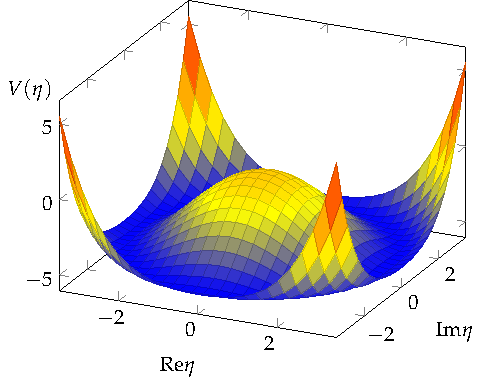
\includegraphics[]{Images/fig-etapotential.pdf}
    \caption{3D plot of the potential $V$ as a function of $\eta$. We take $\mathcal{V} = 1, \mu = 1, \lambda = 1/10$.The blue ring corresponds to $\eta = \sqrt{\frac{\mu}{\lambda}}e^{i\theta}$ which minimizes the potential, which is radially symmetric.}
    \label{fig-etapotential}
\end{figure}

The idea is that the potential is completely symmetric under rotation, but the solution is not. This is something known as spontaneous symmetry breaking. Classical analogy: which way does chalk fall when one lets go of it from the top position. A priori, there is a symmetry; there is no preference to how it falls. But when we actually do the experiment, it falls somewhere as we perturb it somehow when releasing (breaking the symmetry) or an air molecule bounces off of it and causes it to fall. Quantum mechanically, the chalk is described by the rigid rotator Hamiltonian:
\begin{equation}
    H = \frac{I}{2}\dot{\theta}^2
\end{equation}
If I look at the eigenfunctions, we have:
\begin{equation}
    \psi(\theta) = e^{in\theta}
\end{equation}
The ground state is a superposition of all of these angles, which averages out to zero. But this is clearly not the right state; it is in some orientation and it is frozen there. The idea is that the chalk pointing at some angle is actually an excited state; we have something like:
\begin{equation}
    \psi(\theta) = \sum_n e^{in(\theta - \theta_c)}
\end{equation}
and it relaxes towards the ground state given sufficient time; however this time depends on the moment of inertia, which here it is very large. If the chalk was small enough, then we would see it undergo this relaxation; since it is macroscopic, the relaxation time is very large. 

Why this chalk discussion? This is to say that why the quantum mechanical description of the chalk may be correct, it is really not particularly reasonable; it makes more sense to treat this classically.  So, returning back to the idea of spontaneous symmetry breaking. This is a ubiqitous phenomenon (in condensed matter, particle physics, etc.). For example, consider ferromagnetism. The true ground state of a ferromagnetic is some superposition, but if we look at it, it will not decay to the ground state during the lifetime of the universe. So, we can just think about this classically.

Having now chosen a solution, we can't see the symmetry of the whole potential anymore; the fluctuations (as obtained by calculating the higher order terms) cannot ``see'' the whole energy landscape (one can think that the ``moment of inertia'' is so large that it cannot explore the entire ring of minima).

A takeaway from all of this; spontaneous symmetry-breaking is a phenomena we often see when classical effects dominate over quantum ones.

\subsection{Solving the System}
So, we've solved for the leading term of the expansion of $\psi$! Since it's dominant, we could just calculate the internal energy, or the grand canonical free energy from what we have so far. We can find the GC free energy to be:
\begin{equation}
    \varphi = -\frac{\lambda}{2}\rho^2 = -P.
\end{equation}
We can find corrections to this by calculating the contributions from the higher order terms (these corrections should be small, if our asymptotic expansion is actually reasonable). In particular, here this expansion works at low density.

Next, we can plug $\psi = \eta + \tilde{\psi}$ into the field equation (see HW2) or the Hamiltonian (which we do now), and see what we get out. We find:
\begin{equation}
    H' = -\frac{\lambda}{2}\rho^2 V + \int d^3x \left(\frac{\hbar^2}{2m}\nabla \tilde{\psi}^\dag \cdot \nabla \tilde{\psi} + \mu \tilde{\psi}^\dag \tilde{\psi} + \frac{\mu}{2} \tilde{\psi} \tilde{\psi} + \frac{\mu}{2}\tilde{\psi}^\dag \tilde{\psi}^\dag\right) + \O(\lambda)
\end{equation}
Now the Hamiltonian does not look normal in the $\tilde{\psi}$ and $\tilde{\psi}^\dag$s anymore; this is due to the broken symmetry. We can also plug in our expansion into the commutation relations:
\begin{equation}
    [\tilde{\psi}(\v{x}, t), \tilde{\psi}^\dag(\v{y}, t)] = \delta^3(\v{x} - \v{y})
\end{equation}
Let us comment on the $\O(\lambda)$ corrections; we first have that:
\begin{equation}
    -\frac{\lambda}{2}\rho^2V = -\frac{\mu^2}{2\lambda}V
\end{equation}
So this is indeed the leading term for small $\lambda$. The integral term is of order $\lambda^0 = 1$. Then the corrections are of order $\lambda$, so we can control these by taking small $\lambda$.

For large derivatives, the kinetic energy terms dominate, but for smaller derivatives the other terms in the integral become important. 

By plugging things back in, we get a linear field equation for $\tilde{\psi}$ (The Bogolibov-de-Gennes equation); see HW2. But let us attack this Hamiltonian directly:
\begin{equation}
    \psi(\v{x}, 0) = \int \frac{d^3k}{(2\pi)^{3/2}}e^{i\v{k} \cdot \v{x}}\alpha(\v{k})
\end{equation}
this is really just a change of basis in function space; the whole integral is like a unitary matrix that rotates the basis. Let us go to the $\alpha$s; why? Because the Hamiltonian is translation invariant, we would suspect that the momentum would be an important quantity, and $\v{k}$ is closely related to momentum, so it is good to analyze. The Hamiltonian reads:
\begin{equation}
    H = -\frac{\mu^2}{2\lambda}V + \int d^3k \left(\frac{\hbar^2k^2}{2m}\alpha^\dag(\v{k})\alpha(\v{k}) + \mu \alpha^\dag(\v{k})\alpha(\v{k}) + \frac{\mu}{2}\alpha(-\v{k})\alpha(\v{k}) + \frac{\mu}{2}\alpha^\dag(\v{k})\alpha^{\dag}(-\v{k})\right)
\end{equation}
From going to $k$-space, we have a separate Hamiltonian for each value of $\v{k}$, and the first term ($\alpha^\dag(\v{k})\alpha(\v{k})$) is diagonalized. However, it is still not clear what the eigenvalues of the elementary excitations are. We need to diagonalize this Hamiltonian; let us try this. First we note that the Hamiltonian is of quadratic form, so we should be able to diagonalize it. We let:
\begin{equation}\label{eq-bogoliubov}
    \begin{split}
        \alpha(\v{k}) &= \cosh\theta(\v{k})a(\v{k}) - \sinh\theta(\v{k})a^{\dag}(-\v{k})
        \\ \alpha^\dag(\v{k}) &= \cosh\theta(\v{k})a^\dag(\v{k}) - \sinh\theta(\v{k})a(-\v{k})
    \end{split}
\end{equation}
Wait, where do the hyperbolic functions come from? We know that the $\alpha$s follow the commutation relations:
\begin{equation}
    [\alpha(\v{k}), \alpha^\dag(\v{l})] = \delta^3(\v{k} - \v{l})
\end{equation}
so we want the $a$s to do the same:
\begin{equation}
    [a(\v{k}), a^\dag(\v{l})] = \delta^3(\v{k} - \v{l})
\end{equation}
I don't have a lot of freedom in the coefficients if I want the commutation relations to hold; the hyperbolic functions come out of this.

Eqs. \eqref{eq-bogoliubov} is known as a Bogoliubov transformation. We can plug this into the Hamiltonian and get an even more complicated expression with $\sin\theta(\v{k})$s and $a$s, and we can adjust $\theta(\v{k})$ until we get something proportional to $a^\dag(\v{k})a(\v{k})$. When we do so, we end up with:
\begin{equation}
    H = -\frac{\mu^2}{2\lambda}V + \int d^3k E(\v{k})a^\dag(\v{k})a(\v{k}) + E_0
\end{equation}
where the constant at the end comes from the corrections from interchanging the order of operators (as a consistency check: this constant should be small compared to the leading order constant). It is a kind of zero-point energy. In order for the above to hold, we find the constraint that:
\begin{equation}
    \tanh2\theta(\v{k}) = \frac{\mu}{\frac{\hbar^2\v{k}^2}{2m} + \mu}
\end{equation}
and $E(\v{k})$ follows:
\begin{equation}
    E(\v{k}) = \sqrt{\left(\frac{\hbar^2\v{k}^2}{2m} + \mu\right)^2 - \mu^2}
\end{equation}
so we obtain a dispersion relation for $\v{k}$! The cool thing is we can now use this dispersion relation combined with the Landau result to get a testable prediction of the critical velocity for superfluids. For small $\v{k}$, the above reduces to:
\begin{equation}
    E(\v{k}) \approx \sqrt{\frac{\hbar^2}{2m}\mu}\abs{\v{k}}
\end{equation}
So the Landau criterion would tell us that:
\begin{equation}
    v_c = \sqrt{\frac{\hbar^2}{2m}\mu}.
\end{equation}
This turns out to be wrong most of the time, as superfluids are in general not weakly interacting. But, when an experimental group created a weakly-interacting Bose-Einstein condensate, they were able to indeed verify that the above expression holds!

This concludes our discussion; HW2 attacks the same problem from the perspective of the equations of motion.

\subsection{A Small Teaser for Next Lecture}
We've developed our QFT, rewrote many-particle QM as a QFT, and studied some simple (but useful!) examples (such as the Fermi gas\footnote{Quite a useful ``first-order'' approximation for metals.} and superfluids). Now, we go into developing the ideas of QFT a little further. One might wonder why we need something else; this is because this ``something else'' gives us great power and a nicer way to study field theories when we have to do perturbation theory. It may be an unexpected step, but we will temporarily regress from doing QFT to doing classical field theory. We will consider the \emph{action principle}. We will consider some classical field $\psi_\sigma(\v{x}, t)$ (bosons only; anti-commuting fermions would not be pure functions, but would instead be operators belonging to an algebra...). We will then ask if we can derive our field equation from a variational principle and an action. Of course the answer is yes (else we wouldn't bring it up), and we can even write down the Lagrangian density and the action which will yield our classical field equation. The action is:
\begin{equation}
    S = \int dt d^3x \L
\end{equation}
where the Lagrangian density is:
\begin{equation}
    \L = i\hbar \psi^{\dag\sigma}\dpd{}{t}\psi_\sigma - \frac{\hbar^2}{2m}\nabla \psi^{\dag\sigma} \cdot \nabla \psi_\sigma + \mu \psi^{\dag\sigma}\psi_\sigma - \frac{\lambda}{2}\left(\psi^{\dag\sigma}\psi_\sigma\right)^2.
\end{equation}
However, we have lost something: our quantum field equation had a particular ordering of the $\psi$ and $\psi^\dag$s in the interaction part. We have to recover this somehow. This could be a small or large problem; for us it is small because we know how it has to look like ahead of time. But, something like the ordering problem in treating Einstein's gravity is not resolved. In general, this is something one needs to solve case-by-case.

What then, do we gain? The Lagrangian encodes the commutator as well as the field equation. One can encode the first term as:
\begin{equation}
    \left(i\hbar \psi^{\dag\sigma}\right)\left(\dpd{}{t}\psi_\sigma\right) = P\dot{Q}
\end{equation}
and note the connection with the Hamiltonian:
\begin{equation}
    L = P\dot{Q} - H(P, Q).
\end{equation}
One can consider the Poisson bracket:
\begin{equation}
    \{\psi_\sigma(\v{x}, t), i\hbar\psi^{\dag\rho}(\v{y}, t)\} = \delta_\sigma^\rho\delta^3(\v{x} - \v{y})
\end{equation}
and when quantizing one adds an $i\hbar$ and replaces the Poisson bracket with a commutator. So there is that benefit of less writing. We also gain the analysis of symmetries and conserved quantities that we know from classical field theory, which we can lift to the QFT (for example, conservation of energy, momentum).

This is not just a construct; we will learn how to use functional integrals, and the (classical) action plays a very large role there (we integrate over it). It will stay with us for a long time.